\subsection{Hidden Markov Models}

Having examined briefly the theory behind Hidden Markov Models, let us now look at how the training was done offline, and analyse some results from subsequent tests. As mentioned earlier, the apnoeatic states are modelled as the hidden states $\{x_t\}_1^T$, and are elements of the binary set $\{0, 1\}$. The observed signal is annotated every K samples (every minute in the case of the PhysioNet data), so we stack all K samples into $\vec y_t \in \mathbb{R}^d$, ($d = K$). Using the packages \verb!pmtk3! and \verb!HMM Toolbox!, the algorithms were implemented in \verb!MATLAB!\textsuperscript{\textregistered}, along with the conditioning of the data using spectrogram and PCA analysis. Again, \verb!MATLAB!\textsuperscript{\textregistered} is used for convenience and the code can be easily converted to \verb!Java! after experimentation and analysis.

\begin{figure}[h!]
		\centering
			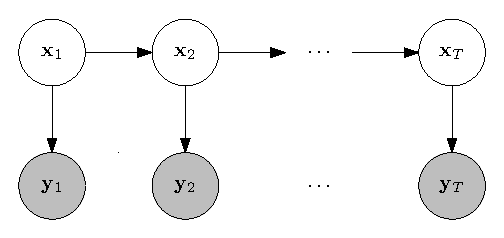
\includegraphics{drawings/pgm.eps}
		\caption{Probabilistic Graphical Model of a SSM and a HMM}
		\label{fig:pgm}
	\end{figure}

We present below parts of the code used for the training and testing of the data, for ease of explanation. Firstly, we present the main script, and subsequently explain the various functions created and used in the script.

\begin{lstlisting}
close all;
clear all;
trainIndex = 1:4;
testIndex = 5:10;

%% Reading and conditioning data
[X, Y, time, signal, annTime] = readData(trainIndex, 1); % X = observations, Y = latent states.
N = 2; % number of states: apnea-noapnea
S = [0; 1]; % set of possible states

%% Transform spectrogram
[XTransformed, YTransformed] = transformSpectrogram(X, Y);
% figure(1);
% hold on;
% plot(time(annTime), Y * 50, 'x');

%% PCA
disp('PCA...');
k = 50; % take k principal components only
[PCoef, PVec, XMean, XVar] = pcaCalc(XTransformed, k);
XPca = pcaTransform(XTransformed, PVec, XMean, XVar);
\end{lstlisting}

The trainIndex and testIndex vector are used simply for selecting the files to be used, out of 35, for training and the remainder (or less) for testing the accuracy of the diagnosis. Having chosen the files, the next step is to extract and read the files. This is done using the readData function, presented below:

\begin{lstlisting}
function [O, q, time, signal, annTime] = readData(fileIndex, keepSignal)

    disp('Reading and conditioning data...');
    filenames = getFilenames();
    
    lastTime = 0;
    annTimeLast = 0;
    time = []; % time
    signal = []; % signal
    annTime = []; % timestamps of annotations
    q = []; % latent states
    O = []; % observations
    for i = fileIndex
        filename = cell2mat(filenames(i));
        disp(sprintf('\tProcessing file %d: %s...', i, filename));
        
        [timeTemp, signalTemp, freq] = rdsamp(filename); % reads the signal
        [annTimeTemp, type] = rdann(filename,'apn'); % reads annotations
        type = (type == 'A');

        %% Conditioning data
        annTimeTemp = [1; annTimeTemp];
        q = [q; type]; % latent states
        for i = 1:length(type)
            O = [O; signalTemp((annTimeTemp(i) + 1):annTimeTemp(i + 1))'];
        end
        
        if keepSignal
            nObs = annTimeTemp(end);
            time = [time; timeTemp(1:nObs) + lastTime + 0.01];
            annTime = [annTime; annTimeTemp(2:end) + annTimeLast];
            signal = [signal; signalTemp(1:nObs)];
            lastTime = time(end);
            annTimeLast = annTime(end);
        end
    end
    if ~keepSignal
        signal = [];
        time = [];
    end
end
\end{lstlisting}

The function reads data from the indices specified in fileIndex (which is trainIndex in the main script above), and returns O, containing all the observations merged together in a TxD matrix. T is the total number of minutes of data, and D is the number of samples in a minute (6000 in this case), such that there are T annotations in total. The function also returns the vector q, a Tx1 vector containing the latent states for every minute in O, as well as consolidated time, signal and annotation time vectors for ease of plotting and analysis later on.

Firstly, readData uses a simple function getFilenames to return a 35x1 cell of the available filenames, in a cell string. Then, after initialising the variables, readData uses a for-loop to run through each file and extract the relevant information. Using the pre-provided rdsamp and rdann functions, the signal values as well as annotations are read from the file. As the annotations use 'A' for apnoeatic episodes and 'N' for non-apnoeatic episodes, the vector type is converted to the alphabet ${0,1}$. The O and q output matrices are built up using the information from each file, and finally some trivial conditioning is done to ensure ease of plotting if the signal were to be kept.

Armed with the consolidated vectors X and Y, we now proceed to use the spectrogram function in \verb!MATLAB!\textsuperscript{\textregistered}, as described in section~\ref{sec:conditioningExperiments}. We then use the \verb!pca! function from the \verb!pmtk3! package to perform Principal Components Analysis (choosing the number of principal components we wish to include, k). 